%Project Documentation
% How does your project work? (Could include the following...)
    % What is its structure?
        % Block and flow diagrams are good here.
    % How does one install your software, if any?
    % How does one run it?
    % Are there any special hardware, OS, or runtime requirements to run your software?
    % Any user guides, API documentation, etc.
    
    
%for code
\lstset{
    frameround=fttt,
    language=bash,
    % numbers=left,
    breaklines=true,
    keywordstyle=\color{black}\bfseries, 
    basicstyle=\ttfamily\color{black},
    numberstyle=\color{black}
    }
    
\subsection{Running the Program on Concept Warehouse}
The webpages are hosted on Concept Warehouse at https://jimi.cbee.oregonstate.edu/concept\_warehouse/. To view the simulation one just needs an internet connection and a web browser. 
Concept Warehouse works in that each simulation is shown in order from Case 1-5 then exploratory mode. To view the simulation, students first predict what is going to happen in the simulation, given the initial state of the pendulum, and then they explain their answer. Students then activate the simulation and then they can press start and view the animation. A live graph update (synced with the simulation) is shown after starting, and live measurements of the height are also shown. Interactions included for the normal mode include the Start, Pause, and Reset button. 
\begin{figure}[H]
  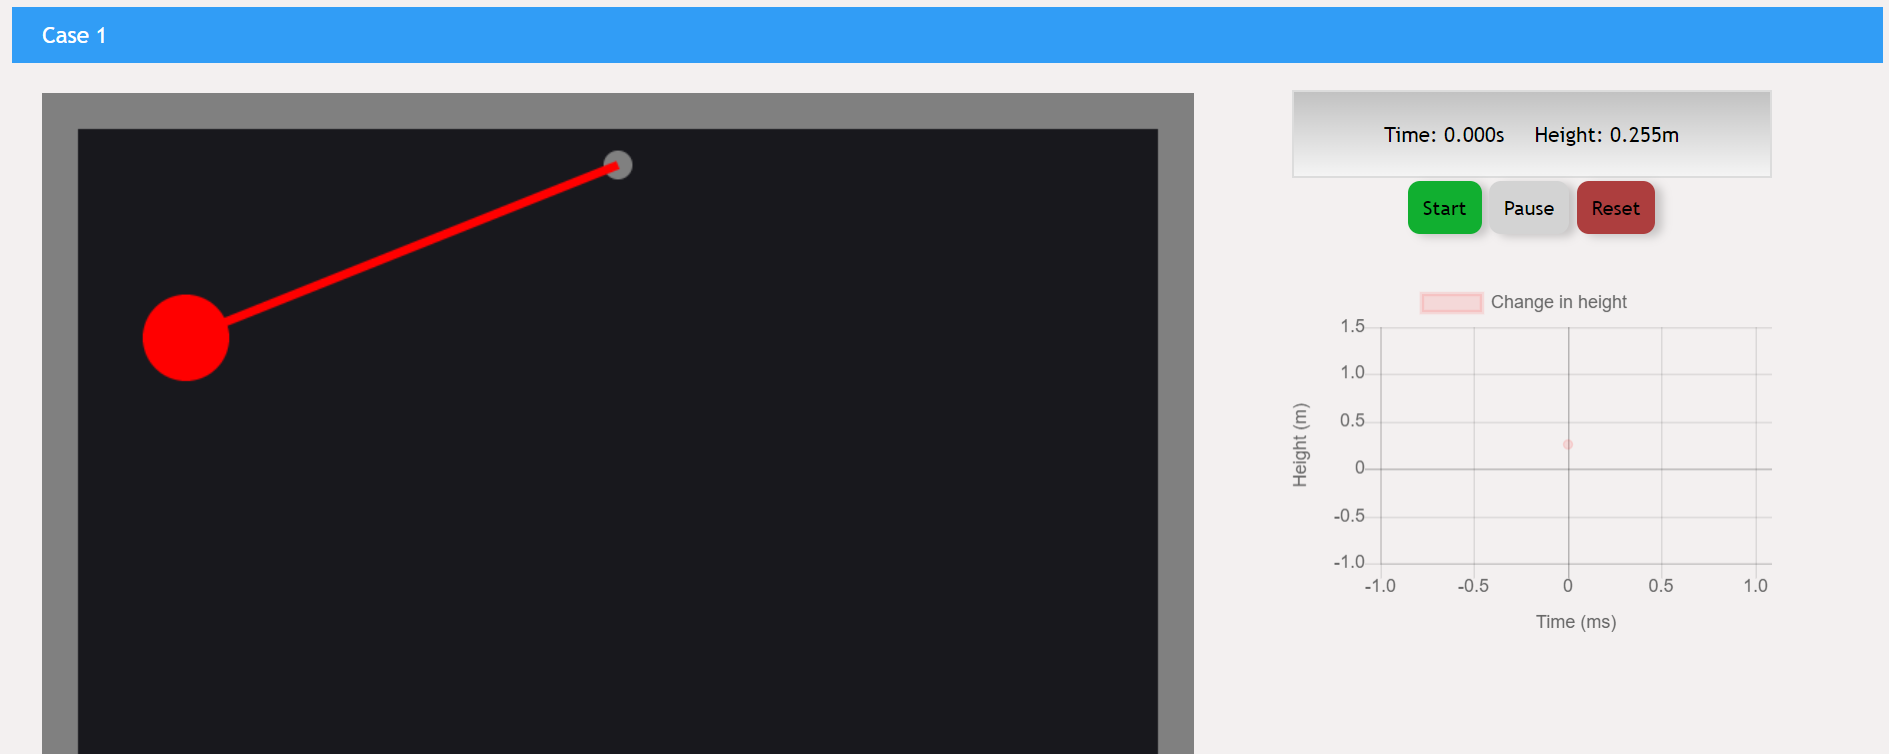
\includegraphics[width=5.5 in]{sim_pics/case1_start.png}
  \caption{Case 1 - initial screen }
  \label{fig:case1_end}
\end{figure}

In Exploratory Mode, users adjust the initial state of the animation using the range sliders on the right - adjusting the number of weights, the graph to be displayed (height/angle/velocity), length, mass, starting angle, and the coefficient of restitution. Then users press start, and the live graph replaces the input sliders. 
\begin{figure}[H]
  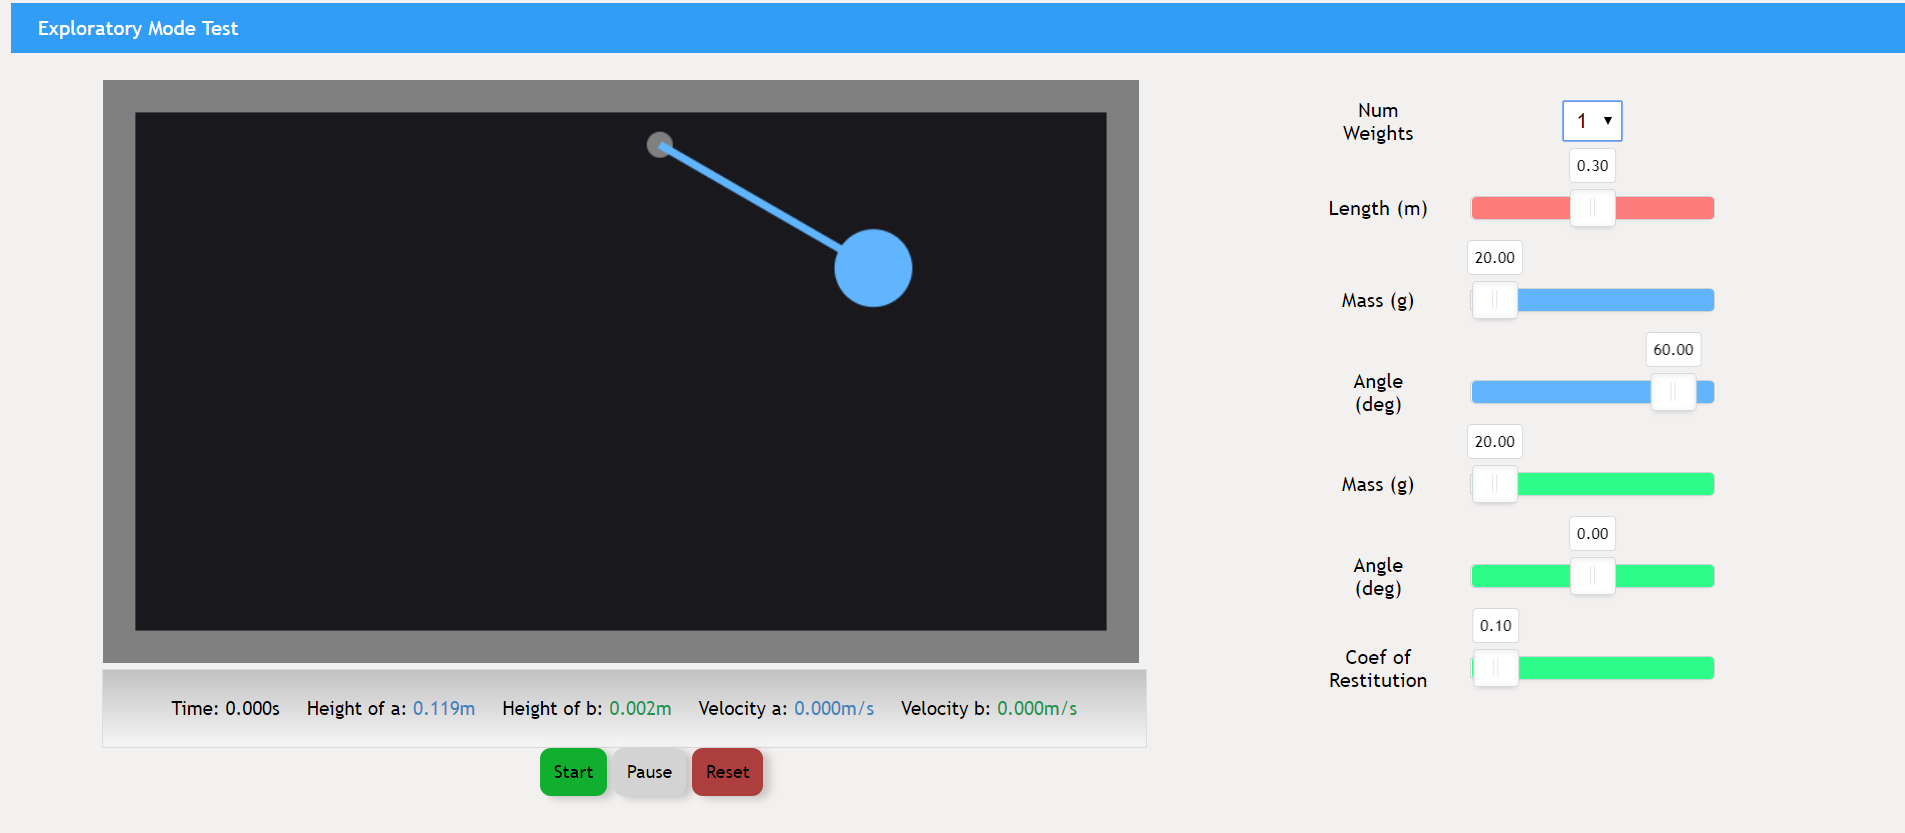
\includegraphics[width=5.5 in]{sim_pics/exploratory_start_1.png}
  \caption{Exploratory Mode - initial screen}
  \label{fig:Exploratory1}
\end{figure}

\subsection{Project Structure}
\subsubsection{Libraries}
These JavaScript libraries are used in the webpage:
\begin{itemize}
    \item Matter.js - Physics library used for the pendulum simulation
    \item Gulp.js - Used for automating build tasks
    \item Chart.js - Used for the graph
    \item noUiSlider - Used to create the range sliders in Exploratory mode
\end{itemize}

\subsubsection{Modules}
There are three basic modules in the project - State, Pendulum, Graph:
\begin{itemize}
    \item The \textbf{State} module handles understanding the current state of the canvas, such as whether it is paused.
    \item The \textbf{Pendulum} module is in charge of keeping tack of the pendulum bodies and properties within the world.
    \item The \textbf{Graph} module handles the state of every graph generated in the project.
\end{itemize}
The sketch.js file in each folder uses these modules with a \lstinline{require} statement and is the starting point for the webpage code.


\subsection{Building the Webpage}
This project uses certain packages to build by using Node as there are different modules used for this project. Make sure node is installed by typing \lstinline{node --version} into the command line. After cloning the repository, run 
\lstinline[columns=fixed]{npm install}
on the command line to install dependencies.
\subsubsection{Building With Gulp}
This project utilizes Gulp to help automate build tasks. In order to install gulp enter
\begin{lstlisting}
    npm install -g gulp-cli
\end{lstlisting}
Once installed, to generate a build folder in the root of the project enter into the command line
\begin{lstlisting}
    gulp
\end{lstlisting}

\noindent This should generate folders case1-case5 and exploratory in the generated build folder. 

\begin{figure}[H]
  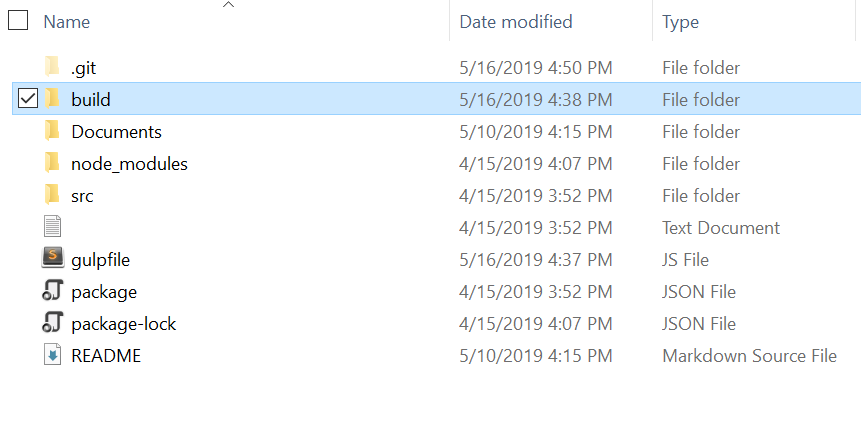
\includegraphics{subfiles/build.PNG}
  \caption{Root Project Structure after gulp command}
  \label{fig:Project}
\end{figure}

\noindent You can then navigate to one of the case folders in the generated build folder (i.e. \lstinline{cd /build/case1}) and enter \lstinline{start index.html} into the command line to view a specific case in the browser.

\begin{figure}[H]
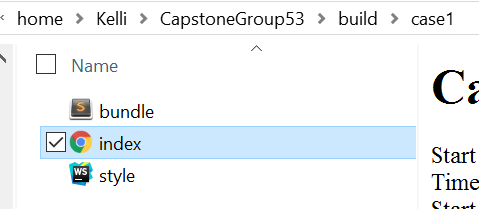
\includegraphics{subfiles/build-case1.PNG}
  \caption{Case folder in /build/case1}
  \label{fig:Case1}
\end{figure}

\noindent Alternatively, in order to build a single case into the build folder located in the root of the project, use the command:
\begin{lstlisting}
    gulp build --case [folder name]
\end{lstlisting}
For example: \lstinline{gulp build --case case2}

\subsubsection{Browserify}
Alternatively, use browserify to manually generate the needed JavaScript file. Navigate to a specific case folder at /src/Pendulum/[case\_folder\_name] (i.e. /src/Pendulum/case2)
and use the command
\begin{lstlisting}
    browserify sketch.js -o bundle.js. 
\end{lstlisting}
After bundle.js is generated, use start index.html to start the webpage in the browser.

